\documentclass[text.tex]{subfiles}

\begin{document}

\begin{definition}
The set $D\subset \CC^n$ such that all points are isolated, that is: 
$$\forall\, z\in D\;\exists\, \epsilon>0:\, B(z,\epsilon)\cap D = \{z\}$$
is a \textbf{discrete set}.
\end{definition}

\section{Delone set} % -------------------------------------------------------------------------------------------------
Delone set is such a set that is both relatively dense and uniformly discrete. These notions are defined using two parameters called packing a covering radius.

\begin{definition}\label{def_deloneSetPacking}
The \textbf{packing radius} of a set $D\subset \CC^n$ is the number: 
$$R_P = \frac{1}{2}\sup\left\{ r_1\in \RR\,\left|\, \forall\, z_1,z_2\in D, z_1\neq z_2:\; \lVert z_1-z_2\rVert >r_1 \right. \right\}$$
\end{definition}

\begin{remark}
Open balls of packing radius centered at the points of the set are disjoint. 
\end{remark}

\begin{definition}\label{def_deloneSetCovering}
The \textbf{covering radius} of a set $D\subset \CC^n$ is the number: 
$$R_C = \inf\left\{ r_2>0\,\left|\, \forall\, z\in\CC^n:\; B(z,r_2)\cap D \neq \emptyset \right. \right\}$$
\end{definition}

\begin{remark}
Union of closed balls of covering radius centered at the points of the set covers the entire space $\CC^n$. 
\end{remark}

\begin{definition}\label{def_deloneSet}
Let $D\subset \CC^n$.\\
If $D$ has positive packing radius $R_P$ then it is \textbf{uniformly discrete}.\\
If $D$ has finite covering radius $R_C$ then it is \textbf{relatively dense}.\\
If $D$ has both positive packing radius $R_P$ and finite covering radius $R_C$ then it is a \textbf{Delone set}.
\end{definition}

\section{Voronoi diagram}\label{sec_voronoi} % ------------------------------------------------------------------------------------------------------
Voronoi diagram is very useful for analysis of local configurations of discrete sets. Since that is essentially the entirety of our work, we define not only the basic Voronoi polygon but also couple nontraditional terms that will ease our work. 

\begin{definition}
Let $P\subset \mathbb{R}^n$ be a discrete set and $x\in P$. The \textbf{Voronoi polygon} or \textbf{Voronoi cell} or \textbf{Voronoi tile} of $x$ on $P$ is the set: 
$$V_P(x) = \{ y \in \mathbb{R}^n \,|\, \forall z \in P, z\neq x:\, \|y-x\|\leq\|y-z\| \}$$
Voronoi polygon $V_P(x)$ is said to \textbf{belong} to the point $x$ and $x$ is called the \textbf{center} of the Voronoi cell $V_P(x)$. 
\end{definition}

\begin{remark}
When there can be no confusion as to what set $P$ is, the index $P$ may be omitted: $V(x)$.
\end{remark}

\begin{definition}
Let $P\subset \mathbb{R}^n$ be a discrete set. The \textbf{Voronoi diagram} or \textbf{Voronoi tessellation} of $P$ is the set: 
$$\{V(x)\,|\, x\in P\}$$
\end{definition}

\begin{definition}
Let $P\subset \mathbb{R}^n$ be a discrete set. The set of centered Voronoi tiles: 
$$\{V(x)-x\,|\, x\in P\}$$
is called the \textbf{list of Voronoi tiles}.
\end{definition}

\begin{remark}
A Voronoi diagram can be viewed as an image whereas a list of Voronoi tiles can be viewed as a list of Voronoi polygon shapes. 
\end{remark}

\begin{definition}
Let $P\subset \mathbb{R}^n$ be a discrete set and let $x\in P$. The \textbf{radius} of Voronoi polygon $V(x)$ is the number: 
$$\sup_{y\in V(x)}\lVert y-x\rVert$$
\end{definition}

\begin{definition}
Let $P\subset \mathbb{R}^n$ be a discrete set and let $x\in P$. The set of points of $P$ that directly shape the Voronoi polygon $V_P(x)$:
$$D_P(x) = \bigcap\, \big\{ Q\subset P\,|\, V_Q(x) = V_P(x) \big\}$$
is called the \textbf{domain} of $x$ or of $V_P(x)$. 
\end{definition}

\begin{figure}[h!]
\centering
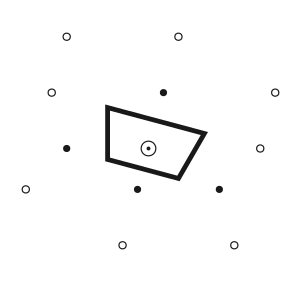
\includegraphics[width=0.36\textwidth]{img/preliminaries/voronoi}
\caption{Example of a Voronoi tile. The set $P$ consists of all the points $\bullet$, $\circ$ and $\odot$. The polygon is the Voronoi cell belonging to the $\odot$ point. The $\bullet$ points are the domain of the Voronoi polygon (i.e. the $\circ$ points do not affect the shape of the Voronoi polygon).}
\label{fig_voronoiExample}
\end{figure}

It will be very useful to explore the Voronoi tessellation on a Delone set. 

\begin{theorem}
Let $P\subset \mathbb{R}^n$ be a Delone set with covering radius $R_C$ and let $x\in P$. Then 
$$V(x)\subset \overline{B(x,R_C)}$$
\end{theorem}
\begin{proof}
By definition of the covering radius (\ref{def_deloneSetCovering}), for any point $y\in \RR^n\setminus \overline{B(x,R_C)}$ there exists $w\in P$ such that $w\in B(y,R_C)$. Therefore $w$ is closer to $y$ than $x$ and so $y\not\in V(x)$.
\end{proof}

\begin{theorem}\label{the_voronoiDomainLimit}
Let $P\subset \mathbb{R}^n$ be a Delone set with covering radius $R_C$ and let $x\in P$. Then 
$$D(x)\subset B(x,2R_C)$$
\end{theorem}
\begin{proof}
For $y\in P$ such that $\lVert y-x \rVert \geq 2R_C$ there exists a point $z\in\RR^n$ such that $\lVert y-z\rVert\geq\lVert x-z\rVert \geq R_C$. Thus if $y$ were in $D(x)$ the Voronoi tile would not be inside $\overline{B(x,R_C)}$. 
\end{proof}

The relationship between a Voronoi polygons and the covering radius is actually even more intricate, as the following theorem shows. 

\begin{theorem}\label{the_voronoiCoveringRadius}
Let $P\subset \mathbb{R}^n$ be a Delone set with covering radius $R_C$ and let $x\in P$. Then the covering radius $R_C$ is the supremum of the radii of the Voronoi tiles:  
$$R_C = \sup_{x\in P}\left\{\sup_{y\in V(x)}\lVert y-x\rVert\right\}$$
\end{theorem}
\begin{proof}
Let us denote the supremum of radii $r= \sup_{x\in P}\left\{\sup_{y\in V(x)}\lVert y-x\rVert\right\}$. We have already proved that $r\leq R_C$. Now assume that $r<R_C$. Then there is a point $y\in\RR^n$ such that $B(y,R_C)~\cap~P~=~\emptyset$ and yet $y\in V(w)$ for some $w\in P$ and thus $\lVert w -y \rVert\leq r$. That is of course a contradiction. 
\end{proof}

\section{Number theory}\label{sec_numberTheory} % -------------------------------------------------------------------------------------------------
The study of quasicrystals relies heavily on number theory. Therefore this section lists definitions and their corollaries that are used further. For proofs of our claims we refer the reader to \cite. 
\begin{definition}
Let $P\subset\CC$. The ring of polynomials in $x$ with coefficients in $P$ is denoted by $P[x]$. 
\end{definition}

\begin{definition}
Polynomial $f\in\CC[x]$ such that $f(x) = \sum_{k=0}^m{\alpha_kx^k}$ for some $m\in\NN$, where $\alpha_m = 1$ is a \textbf{monic polynomial}. 
\end{definition}

\begin{definition}
Polynomial $f\in\CC[x]$ such that $\forall\, g,h\in\CC[x]:\;f \neq gh$ is an \textbf{irreducible polynomial}. 
\end{definition}

\subsection{Algebraic numbers, minimal polynomial and degree}
\begin{definition}Let $\alpha, \beta\in\CC$.\\
If there exists a monic polynomial $f\in\QQ[x]$ such that $f(\alpha) = 0$, then $\alpha$ is an \textbf{algebraic number}. The set of algebraic numbers is denoted as $\AAA$. \\
If there exists a monic polynomial $g\in\ZZ[x]$ such that $g(\beta) = 0$, then $\beta$ is an \textbf{algebraic integer}.  The set of algebraic integers is denoted as $\BB$. 
\end{definition}

\begin{definition}
Irreducible monic polynomial $f\in\QQ[x]$ of the smallest degree such that $f(\alpha) = 0$ for $\alpha\in\AAA$ is the \textbf{minimal polynomial} of $\alpha$. It is usually denoted as $f_\alpha$.
\end{definition}

\begin{definition}
The \textbf{degree} of an algebraic number is the degree of its minimal polynomial. 
\end{definition}

\begin{remark}
For each algebraic number there exists exactly one minimal polynomial. 
\end{remark}

\subsection{Galois isomorphism}

\begin{definition}
Let $\alpha\in\AAA$ of degree $m$ and $f_\alpha\in\QQ[x]$ be its minimal polynomial. The $(m-1)$ other roots of $f_\alpha$ are called \textbf{conjugate roots} of $\alpha$ and are denoted as $\alpha^{(1)},\,\alpha^{(2)},\,\dots,\,\alpha^{(m-1)}$. 
\end{definition}

\begin{remark}
Consistently with the notation of its conjugate roots, $\alpha$ may be denoted as $\alpha^{(0)}$ or $\alpha^{(m)}$.
\end{remark}

\begin{remark}
For low degrees the upper indexes are often written in unary -- e.g. $\alpha, \alpha', \alpha''$. 
\end{remark}

\begin{definition}
Let $\alpha\in\AAA$ of degree $m$. The \textbf{extension ring} of the number $\alpha$ is the set: 
$$\ZZ(\alpha) = \left\{ a_0 + a_1\alpha + a_2\alpha^2 + \dots + a_{m-1}\alpha^{m-1} \left |\; a_i\in\ZZ\right. \right\}$$
\end{definition}

\begin{definition}
Let $\alpha\in\AAA$ of degree $m$. The \textbf{extension field} of the number $\alpha$ is the set: 
$$\QQ(\alpha) = \left\{ b_0 + b_1\alpha + b_2\alpha^2 + \dots + b_{m-1}\alpha^{m-1} \left |\; b_i\in\QQ\right. \right\}$$
\end{definition}

\begin{remark}
Extension ring of $\alpha$ is the smallest ring containing $\alpha$ as well as all integers. 
Extension field of $\alpha$ is the smallest field containing $\alpha$ as well as all rationals. 
\end{remark}

\begin{definition}
Let $\alpha\in\AAA$ of degree $m$ and let $\alpha^{(1)},\,\alpha^{(2)},\,\dots,\,\alpha^{(m-1)}$ be its conjugate roots. Then $\QQ(\alpha),\, \QQ(\alpha'),\,\dots,\, \QQ(\alpha^{(m-1)})$ are isomorphic. The \textbf{Galois isomorphisms} are:
$$\sigma_i:\,\QQ(\alpha)\to\QQ\big(\alpha^{(i)}\big)\quad\text{induced by}\quad\sigma_i(\alpha) = \alpha^{(i)}\qquad i\in\widehat{m-1}$$
\end{definition}

Galois isomorphisms play a significant role in the definition of the quasicrystals, so they surely deserve an example. 

The Galois isomorphism $\sigma_0$ is always identity.

In general the Galois isomorphism $\sigma_i$ exchanges $\alpha$ of degree $m$ with its $i$th conjugate root. 
$$\sigma_i\big(b_0 + b_1\alpha + b_2\alpha^2 + \dots + b_{m-1}\alpha^{m-1}\big) = b_0 + b_1\alpha^{(i)} + b_2\big(\alpha^{(i)}\big)^2 + \dots + b_{m-1}\big(\alpha^{(i)}\big)^{m-1}$$

Since further we will only work with quadratic algebraic numbers (i.e. of degree $2$), there will only be two roots of a given minimal polynomial, $\alpha$ and $\alpha'$, and two Galois isomorphisms, namely the identity and $\sigma_1(\alpha) = \alpha'$. Moreover, $\alpha'\in\QQ(\alpha)$, thus $\sigma_1$ is an automorphism of the quadratic field $\QQ(\alpha)$ and is often denoted only as $'$ -- i.e. $\sigma_1(x) = x'$ for $x\in\QQ(\alpha)$.

\subsection{Root of unity, cyclotomic polynomial}\label{sec_rootOfUnity}

\begin{definition}
Every $\zeta\in\CC$ such that $\zeta^n-1=0$ for $n\in\NN$ is called the \textbf{$n$th root of unity} or just \textbf{root of unity} if $n$ is not given. Minimal $d\in\NN$ for which $\zeta^d-1=0$ is the \textbf{order} of $\zeta$. \\
Nontrivial root of unity is different from one. 
\end{definition}

\begin{remark}
Nontrivial root of unity is a root of polynomial $\frac{x^n-1}{x-1}$.
\end{remark}

\begin{remark}
$n$th root of unity may be written as $\zeta = e^{2k\pi \i/n}$ for $k\in \{0, 1, \dots, n-1\}$.
\end{remark}

\begin{theorem}
Degree of $n$th root of unity $\zeta$ is $\varphi(n)$, where $\varphi$ is the Euler function.
\end{theorem}

Now we would like to look at the Galois isomorphisms of $n$th root of unity $\zeta$ of degree $4$. It will be evident why $4$ later. By previous theorem, that means $\varphi(n)=4$. 

The three conjugate roots of $\zeta$ are also $n$th roots of unity and as such they are powers of $\zeta$, specifically $\{\zeta^k\,|\,k\bot n, k>1\}$. 

Since $k\bot n$ implies $(n-k)\bot n$ and also
$$\cos\left(\frac{2k\pi}{n}\right) = \cos\left(\frac{2\left(n-k\right)\pi}{n}\right) \quad\text{and}\quad \sin\left(\frac{2k\pi}{n}\right) = -\sin\left(\frac{2\left(n-k\right)\pi}{n}\right)$$
the four roots $\zeta^{(0)}, \zeta^{(1)}, \zeta^{(2)}, \zeta^{(3)}$ appear in pairs of complex conjugates. Therefore among the four Galois isomorphisms there are two that do not change the real part of $\zeta$ and two that do change it. This will become very significant once we introduce the Pisot-cyclotomic numbers. 

\subsection{Pisot numbers}
\begin{definition}
Let $\beta\in\BB$ be an algebraic integer of degree $m$, $\beta>1$  and for all conjugate roots $\beta',\,\beta'',\,\dots ,\,\beta^{(m-1)}$ it holds
$$|\beta^{(i)}|<1\qquad \forall\, i\in\widehat{m-1}$$
Then $\beta$ is called \textbf{Pisot} number.
\end{definition}

As we will see in Section \ref{sec_pisotCyclotomic}, Pisot numbers represent another crucial notion to our quasicrystal model. 

\subsection{Vieta's formulas}
Since we will work a lot with roots of quadratic equations we want to, just for completeness, show the Vieta's formulas in the form in which we will use them. 

The roots $x,x'\in\CC$ of quadratic polynomial $ax^2+bx+c$ satisfy: 
$$x+x'=-\frac{b}{a}\qquad\text{and}\qquad xx'=\frac{c}{a}$$

For a monic quadratic polynomial ($a=1$) we have:
$$x+x'=-b\qquad\text{and}\qquad xx'=c$$

We will often want to express one root in terms of the other: 
$$x=-b-x'\qquad\text{and}\qquad x=\frac{c}{x'}$$


\section{Crystallography}\label{sec_crystallography}% -------------------------------------------------------------------------------------------------
Even though we are further going to work only with quasicrystals, they are often described by their differences from crystals. Therefore we briefly touch on the very basics of crystallography. 

A lattice is usually used as a model for a crystal. 

\begin{definition}
Let $\{\mathbf{e}_1, \dots, \mathbf{e}_d\}$ be a basis of $\RR^d$ for $d\in\NN$. \textbf{Lattice} in $\RR^d$ is the set
$$L = \bigoplus^d_{j=1}\ZZ\, \mathbf{e}_j$$
\end{definition}

There is an important theorem in crystallography, the crystallographic restriction theorem, that limits the rotational symmetries available to crystals. Here we only show the two dimensional variant. 

\begin{theorem}
Two dimensional lattices are limited to 2-fold, 3-fold, 4-fold, and 6-fold rotational symmetries. 
\end{theorem}

These rotational symmetries, 2-fold, 3-fold, 4-fold, and 6-fold, are thus called \textbf{crystallographic} rotational symmetries. 

Quasicrystals are of course not bounded by the crystallographic restriction theorem and therefore have different rotational symmetries, we will call these different rotational symmetries \textbf{non-crystallographic}.

\section{Cut-and-project scheme}\label{sec_cutAndProject}% -------------------------------------------------------------------------------------------------
We are using cut-and-project scheme to model the quasicrystals. Here is a brief introduction into its workings. In general, cut-and-project is a specific way of selecting a subset from a larger set.

The cut-and-project scheme utilizes $m+n$ dimensional lattice $L\subset\RR^{m+n}$, $m$ dimensional subspace $V_1\subset\RR^{m+n}$ and $n$ dimensional subspace $V_2\subset\RR^{m+n}$. Further we define two projections $\pi_1:\RR^{m+n}\rightarrow V_1$ and $\pi_2:\RR^{m+n}\rightarrow V_2$ such that $\pi_1|_L$ is injection and $\pi_2(L)$ is dense in $V_2$. 

These projections are where the 'project' part of the cut-and-project scheme comes from. The 'cut' part comes from a bounded subset $\Omega\subset V_2$ with nonempty interior usually referred to as \textbf{window}. 

All put together the cut-and-project scheme produces a subset $Q\subset \pi_1(L)$:
$$Q = \{ \pi_1(x)\; |\; \pi_2(x)\in \Omega,\,  x\in L \}$$
Put in words the set $Q$ are $\pi_1$ projections of those points of $L$ whose $\pi_2$ projections fit in the window $\Omega$. 

The notation can be somewhat simplified by composing a projection between $\pi_1(L)$ and $\pi_2(L)$:~$\pi_2\circ\pi^{-1}_1$, usually denoted as $\ast$ and referred to as the \textbf{star map}. $Q$ then becomes:
$$Q = \{ x \in V_1\; |\; x^\ast\in \Omega \}$$
This is the form in which we will use the cut-and-project scheme. 
\end{document}
